\documentclass{beamer}
\usepackage{etex}
\reserveinserts{28}
\usepackage[utf8]{inputenc}
\usepackage[T1]{fontenc}
\usepackage{xspace}
% \usepackage[colorlinks=true]{hyperref}
\usepackage{color}

\usepackage{amsmath}
\usepackage{amssymb,amsthm,amsfonts}
\usepackage{mathbbol}
\usepackage{pgfplots}
\newtheorem{thm}{Theorem}
\newtheorem{cor}[thm]{Corollary}
\newtheorem{prop}[thm]{Proposition}
\newtheorem{defi}[thm]{Definition}
\newtheorem{lem}[thm]{Lemma}
\newtheorem{ax}[thm]{Axiom}

\newcommand \defeq {\overset{de\hspace{-0.2ex}f}{=}}

\newcommand{\mynote}[2]{
  \fbox{\bfseries\sffamily\scriptsize#1}
  {\small$\blacktriangleright$\textsf{\emph{#2}}$\blacktriangleleft$}~}

\newcommand\kq[1]{\mynote{KQ}{#1}}
\newcommand\nt[1]{\mynote{NT}{#1}}

\newcommand{\ie}{i.e,\xspace}
\newcommand{\eg}{e.g,\xspace}

% correct bad hyphenation here
\hyphenation{op-tical net-works semi-conduc-tor}


\usepackage{enumerate}
\usepackage{wasysym}

\mode<beamer>{%
  \usetheme[right,width=0mm]{Goettingen}
}

\AtBeginSection[]{
  \begin{frame}<beamer>{}
    \tableofcontents[currentsection,currentsubsection]
    \note{ }
  \end{frame}
}

\setbeamertemplate{navigation symbols}{} 
\usepackage{pgfpages}
\setbeameroption{show notes on second screen=right}

\usepackage{bussproofs}


\usepackage[all]{xy}
\def\dar[#1]#2{\ar@<-#2>[#1]\ar@<#2>[#1]} %double arrows in xy
\def\tar[#1]#2{\ar@<#2>[#1]\ar@<0pt>[#1]\ar@<-#2>[#1]} %triple arrows in xy
\DeclareMathOperator{\Type}{Type}
\DeclareMathOperator{\HProp}{HProp}
\DeclareMathOperator{\HSet}{HSet}
\DeclareMathOperator{\IsHProp}{IsHProp}
\DeclareMathOperator{\IsHSet}{IsHSet}
\DeclareMathOperator{\nat}{nat}
\DeclareMathOperator{\Unit}{Unit}
\DeclareMathOperator{\im}{Im}
\DeclareMathOperator{\id}{id}
\DeclareMathOperator{\Contr}{Contr}
\DeclareMathOperator{\IsContr}{IsContr}
\DeclareMathOperator{\IsEquiv}{IsEquiv}
\DeclareMathOperator{\precompose}{\mathrm{precompose}}
\DeclareMathOperator{\postcompose}{\mathrm{postcompose}}
\DeclareMathOperator{\idmap}{\mathrm{idmap}}
\DeclareMathOperator{\cocone}{cocone}
\DeclareMathOperator{\inl}{inl}
\DeclareMathOperator{\inr}{inr}
\DeclareMathOperator{\transport}{transport}
\DeclareMathOperator{\tr}{tr}
\DeclareMathOperator{\Sym}{Sym}
\DeclareMathOperator{\Trans}{Trans}
\DeclareMathOperator{\Refl}{Refl}


\def\mymathhyphen{{\hbox{-}}}

\newcommand{\IsType}[1]
{\mathop{\mathrm{Is\mymathhyphen}#1\mathrm{\mymathhyphen type}} }

\newcommand{\modal}{\ensuremath{\ocircle}}
\newcommand \True {\top}
\newcommand \idpath {\mathrm{idpath}}
\newcommand \False {\bot}
\newcommand \closure[1] {\overline{#1}}
\newcommand \Char[1] {\chi_{#1}}%{\mathrm{char}(#1)}
\newcommand \E {\mathcal{E}}
\newcommand \Hom[1] {\mathrm{Hom}_{#1}}
\newcommand \Obj {\mathrm{Obj}}
\newcommand \Sh[1] {\mathrm{Sh}_{#1}}
\newcommand \squash[1] {\| #1 \| }
\newcommand \separated {\mathop{\square_{n+1}} }
\newcommand \fib[2] {\mathrm{fib}_{#1}(#2)}
\newcommand \colim {\mathrm{colim}}
\newcommand \zero {\mathbf{0}}
\newcommand \one {\mathbf{1}}
\newcommand \unittt{\star}
\newcommand \two {\mathbf{2}}
\newcommand{\sumD}[3]{\sum_{#1:#2}\, #3}
\newcommand{\prodD}[3]{\prod_{#1:#2}\, #3}
\newcommand{\homot}{\sim}
\newcommand{\retr}{\mathrm{retr}}
\newcommand{\sect}{\mathrm{sect}}
\newcommand{\adj}{\mathrm{adj}}
\newcommand{\ap}[1]{\mathrm{ap}_{#1}}
\newcommand{\inv}[1]{#1^{-1}}
\newcommand{\concat}[2]{#1\cdot #2}
\newcommand{\happly}{\mathrm{happly}}
\newcommand{\Sone}{\mathbb{S}^1}
\newcommand{\baseS}{\mathrm{base}}
\newcommand{\loopS}{\mathrm{loop}}
\newcommand{\coeq}[2]{\mathrm{Coeq}^{#1,#2}}
\newcommand{\nType}[1]{\Type_{#1}}

\DeclareMathOperator{\issep}{IsSeparated}
\DeclareMathOperator{\issheaf}{IsSheaf}
\DeclareMathOperator{\KP}{KP}
\DeclareMathOperator{\kp}{kp}

\addtobeamertemplate{footline}{\insertframenumber/\inserttotalframenumber}

\title[Sheafification in HoTT]{Lawvere-Tierney Sheafification\\ in Homotopy Type Theory}

\author[]{{Kevin Quirin} \\ 
  {Mines de Nantes \\ Nantes, France}}

\date{13 December 2016}

\usepackage{tikz}

\begin{document}

\begin{frame}
    
    \note{Thank you all for coming, especially the members of the
      committee. It is a great honour for me to have such a great
      comittee for my defence.

    I will present you my work on sheafification in homotopy type theory}
    \maketitle
    
\end{frame}

\section[Type Theory]{Introduction to type theory}
\label{sec:intr-type-theory}

\subsection[Proof]{Formalizing proofs}
\label{sec:formalizing-proofs}

\begin{frame}
  \frametitle{Errors in mathematics}
  
  One issue with mathematics: it is hard to check proofs.
  \onslide<2->{
    \begin{center}
    

  % \begin{center}
    \frame{
      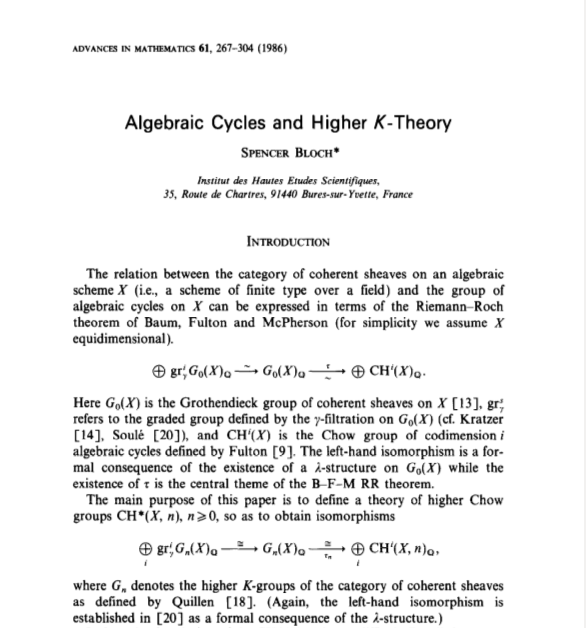
\includegraphics[scale=0.3]{spencer_bloch}}
    \note[item]{In a paper by Spencer Bloch, Suslin found an error in lemma
      1.1. Almost all the paper ws relying on this lemma}
  % \end{center}
  \llap{%
    % \begin{center}
    \frame{\includegraphics<3,4>[scale=0.35]{bloch_lemma}}
    % \end{center}
  }}
  \end{center}
  \note<2->[item]{While the original - false - proof was only a few lines long,
    the new proof is about thirty pages long, and contains complex
    arguments.}
  \note<4->[item]{We would like the proof to be checked by an
    automatic process, by computers, to avoid human mistakes}
  \onslide<4>{
    Proofs are more and more complicated.
  }

\end{frame}

% \begin{frame}[c]
%   \centering


%   \note<1->[item]{If you give a proof to the best mathematician}
%   \note<2->[item]{He will probably don't know if it is true or not}
%   \note<3->[item]{Our hope is to give to rather to a computer}
%   \note<4->[item]{Who can decide if it is right or wrong, and in the
%     latter case, where is the error}
%   \begin{tabular}{ccc}
%   % \begin{center}
%     \onslide<1,3>{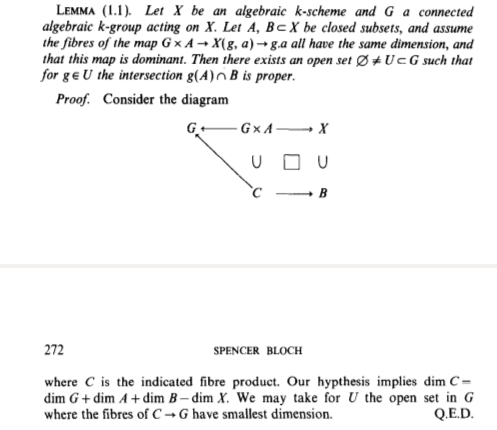
\includegraphics[scale=0.15]{bloch_lemma}} &
%     \only<1,2>{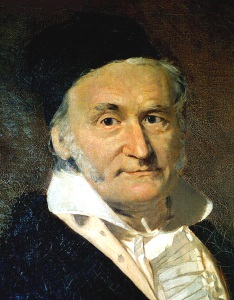
\includegraphics[scale=0.7]{gauss}}
%     \only<3,4>{
\includegraphics[scale=0.25]{computer}
      
% }
%       &
%       \begin{overprint}
%         \onslide<2>{\quad\Large Ich wei\ss{} nicht }
%         \onslide<4>{\hspace{-8em}\begin{tabular}[x]{@{}c@{}}False\\Error
%             on line 4\end{tabular}}
%       \end{overprint}

    
%   % \end{center}
%   \end{tabular}
% \end{frame}

\subsection[Curry-Howard]{The Curry-Howard isomorphism}
\label{sec:curry-howard-isom}

\begin{frame}
  \frametitle{Curry-Howard}
  
  As the previous section suggests, it is a good idea to know what is
  a correct proof.

  \vspace{2em}
  This part of mathematics is called {\em proof theory}.

  \vspace{2em}
  It describes how to be sure that a proof is correct.
\end{frame}

\begin{frame}

  \begin{center}
    \AxiomC{}
    \UnaryInfC{$\Gamma\vdash \top$}
    \DisplayProof
    \qquad
    \AxiomC{$\Gamma,A\vdash B$}
    \UnaryInfC{$\Gamma \vdash A \Rightarrow B$}
    \DisplayProof
  \end{center}
\begin{center}
    \AxiomC{$\Gamma \vdash A$}
    \AxiomC{$\Gamma \vdash B$}
    \BinaryInfC{$\Gamma \vdash A\land B$}
    \DisplayProof
  \end{center}
  \begin{center}
    \AxiomC{$\Gamma\vdash A$}
    \UnaryInfC{$\Gamma\vdash A\lor B$}
    \DisplayProof
    \qquad
    \AxiomC{$\Gamma \vdash B$}
    \UnaryInfC{$\Gamma\vdash A\lor B$}
    \DisplayProof
  \end{center}
  \begin{center}
    \AxiomC{$\Gamma\vdash A$}
    \AxiomC{$\Gamma\vdash A\Rightarrow B$}
    \BinaryInfC{$\Gamma\vdash B$}
    \DisplayProof
  \end{center}
\end{frame}

\begin{frame}
  These rules really look like the ones of lambda-calculus, the most
  simple programming language~: 

    \begin{center}
    \AxiomC{}
    \UnaryInfC{$\Gamma\vdash \onslide<2>{\unittt\,:\,} \top$}
    \DisplayProof
    \qquad
    \AxiomC{$\Gamma,\onslide<2>{a\,:\,}A\vdash \onslide<2>{b\,:\,}B$}
    \UnaryInfC{$\Gamma \vdash A \Rightarrow B$}
    \DisplayProof
 \end{center}
\begin{center}
    \AxiomC{$\Gamma \vdash \onslide<2>{a\,:\,}A$}
    \AxiomC{$\Gamma \vdash  \onslide<2>{b\,:\,}B$}
    \BinaryInfC{$\Gamma \vdash \onslide<2>{(a,b)\,:\,} A\land B$}
    \DisplayProof
  \end{center}
  \begin{center}
    \AxiomC{$\Gamma\vdash \onslide<2>{a\,:\,}A$}
    \UnaryInfC{$\Gamma\vdash \onslide<2>{\inl a\,:\,}A\lor B$}
    \DisplayProof
    \qquad
    \AxiomC{$\Gamma \vdash \onslide<2>{b\,:\,} B$}
    \UnaryInfC{$\Gamma\vdash \onslide<2>{\inr b\,:\,}A\lor B$}
    \DisplayProof
  \end{center}
  \begin{center}
    \AxiomC{$\Gamma\vdash\onslide<2>{a\,:\,} A$}
    \AxiomC{$\Gamma\vdash\onslide<2>{f\,:\,} A\Rightarrow B$}
    \BinaryInfC{$\Gamma\vdash\onslide<2>{f\,a\,:\,} B$}
    \DisplayProof
  \end{center}
\end{frame}

\begin{frame}
  The Curry-Howard isomorphism states that there are correspondances:
  \begin{itemize}
  \item Type $\leftrightsquigarrow$ Formula
  \item Term/program $\leftrightsquigarrow$ Proof
  \item Type-checking $\leftrightsquigarrow$ Verification of proof
  \end{itemize}
\end{frame}

\section[Forcing]{Forcing, Sheafification and Translation}
\label{sec:forc-sheaf}

\subsection[ZFC]{Forcing in set theory}
\label{sec:forcing-set-theory}

\begin{frame}{Forcing in set theory}
  \note<1->[item]{I'll explain it briefly on a schema}
  \note<2->[item]{Let M be a model of ZFC, with its ordinal numbers}
  \note<3->[item]{We want a new model MG, sharing the same ordinals as
  M, but containing a witness of the desired property}
  \note<4->[item]{We reach it from within M with approximations of it,
  contained in a set P (called the forcing condition). 

  In MG, P contains a subset G, called a generic element, and its
  limit is the desired witness}


  In set theory, forcing is a way to extend a model of ZF(C) with new
  witnesses for formulas, \eg{} {\em continuum hypothesis}.
  \begin{center}
  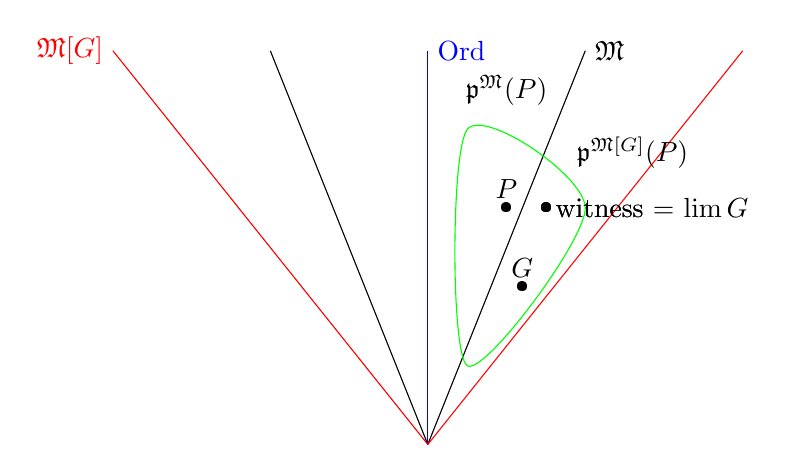
\begin{tikzpicture}
    \onslide<2->{
      \draw (0,0) -- (-2,5);
      \draw (0,0) -- (2,5) node[right] {$\mathfrak M$};
      \draw[color=blue] (0,0) -- (0,5) node[right] {Ord};}
    \onslide<3->{
      \draw[color=red] (0,0) -- (-4,5) node[left] {$\mathfrak M[G]$};;
      \draw[color=red] (0,0) -- (4,5);}
    \onslide<4->{
      \draw [green] plot [smooth cycle] coordinates {(0.5,1) (0.5,4)
        (2,3)};
      \draw (1,4.5) node {$\mathfrak p^{\mathfrak M} (P)$};
      \draw (2.6,3.7) node {$\mathfrak p^{\mathfrak M[G]} (P)$};
      \draw (1,3) node {\textbullet};
      \draw (1,3) node[above] {$P$};
      \draw (1.2,2) node {\textbullet};
      \draw (1.2,2) node[above] {$G$};
      \draw (1.5,3) node {\textbullet};
      \draw (1.5,3) node[right] {witness = $\lim G$};}
    \onslide<3>{
      \draw (1.5,3) node {\textbullet};
      \draw (1.5,3) node[right] {witness};}
  \end{tikzpicture}
  \end{center}
\end{frame}

\subsection[Sheafification]{Sheafification in a topos}
\label{sec:sheafification-topos}

\begin{frame}{Recall: Sheafification in topos}
  \note{ }
  Let $j$ be a Lawvere-Tierney topology on a topos $\mathcal T$, with
  subobject classifier $\Omega$.

  \only<5>{
  $$\xymatrix @!0 @C=4pc @R=3pc {
    T \ar[rr]^{\{\cdot\}_T} \ar@{->>}[d]_-{\mu_T} && \Omega^T \ar[d]^-{j^T}  &
    \\
    \im \left(j^T \circ \{\cdot\}_T \right) \ar@{^{(}->}[rr]^-{\text{mono}} \ar[rd] && \left( \Omega_j
    \right)^T & \ar@{~>}@*{[blue]}[l] \text{\textcolor{blue}{sheaf}}\\
    & \mathfrak a
    (T) \defeq \overline{\im \left(j^T \circ \{\cdot\}_T \right)} \ar[ur] & & \ar@{~>}@*{[blue]}[ll] \text{\textcolor{blue}{sheaf}} \\
    \text{\textcolor{blue}{separated}} \ar@/^2pc/@{~>}@*{[blue]}[uu]
  } $$}

  \only<2>{
  $$\xymatrix @!0 @C=4pc @R=3pc {
    T \ar[rr]^{\{\cdot\}_T} && \Omega^T \ar[d]^-{j^T}  &
    \\
    && \left( \Omega_j
    \right)^T &\\
    &\\
  } $$}

  \only<3>{
  $$\xymatrix @!0 @C=4pc @R=3pc {
    T \ar[rr]^{\{\cdot\}_T} \ar@{->>}[d]_-{\mu_T} && \Omega^T \ar[d]^-{j^T}  &
    \\
    \im \left(j^T \circ \{\cdot\}_T \right) \ar@{^{(}->}[rr]^-{\text{mono}} && \left( \Omega_j
    \right)^T & \\
    & \\
  } $$}

  \only<4>{
  $$\xymatrix @!0 @C=4pc @R=3pc {
    T \ar[rr]^{\{\cdot\}_T} \ar@{->>}[d]_-{\mu_T} && \Omega^T \ar[d]^-{j^T}  &
    \\
    \im \left(j^T \circ \{\cdot\}_T \right) \ar@{^{(}->}[rr]^-{\text{mono}} \ar[rd] && \left( \Omega_j
    \right)^T & \\
    & \mathfrak a
    (T) \defeq \overline{\im \left(j^T \circ \{\cdot\}_T \right)} \ar[ur] & & \\
  } $$}


  \only<2>{Send $T$ to $\Omega^T$ via the singleton map, then postcompose with
    $j:\Omega \to \Omega_j$}
  \only<3>{Compute the image of this map: it is a subobject of $\left(
      \Omega_j \right)^T$ \phantom{xxxxxxxxxxxxxxxxxxxxxxxxxxxxxxx}}
  \only<4>{Close this subobject \phantom{xxxxxxxxxxxxxxx
      xxxxxxxxxxxxxxxx xxxxxxxxxxxxxxxx }}
  \only<5>{Key points:
  \begin{itemize}
  \item $\left( \Omega_j \right)^T$ has to be a sheaf.
  \item A closed subobject of a sheaf should be a sheaf.
  \end{itemize}
}
\end{frame}

\begin{frame}
  \begin{center}
    \[
    \begin{array}{ccc}
      \text{Topos }\mathcal T &
      \onslide<2->{\xrightarrow{\qquad\mathfrak a\qquad}} &
      \onslide<2->{\text{Sheaf topos } \Sh{\lnot\lnot}(T)} \\
        && \\
        \text{Axioms of topos} & \onslide<2->{\xrightarrow{\qquad~\qquad}}
        &\onslide<2->{
          \begin{array}{l}
            \text{Axioms of topos} \\ \text{+ Law of Excluded Middle}
            \\ \text{+ Axiom of Choice}
          \end{array}
          }
    \end{array}
    \]
  \end{center}
\end{frame}

\subsection{Translations}
\label{sec:translations}

\begin{frame}
  \frametitle{Gödel-Gentzen translation}
  \only<1>{
    From classical logic to intuitionistic logic:
    \begin{center}
      \[
      \begin{array}{rcl}
        \phi^N & \mapsto & \lnot\lnot \phi \\
        && \\
        (\phi\land\psi)^N &\mapsto & \phi^N \land \psi^N \\
        &&\\
        (\phi \lor \psi)^N & \mapsto & \lnot (\lnot \phi^N \land
        \lnot\psi^N) \\
        && \\
        (\forall x,\, \theta(x))^N &\mapsto & \forall x,\,
        (\theta(x))^N \\
        && \\
        (\exists x,\, \theta(x))^N & \mapsto & \lnot (\forall x,\, \lnot(\theta(x))^N)
      \end{array}
      \]
    \end{center}
  }
  \only<2>{
    \begin{center}
      \[
      \begin{array}{rcl}
        \phi & \mapsto & \phi^N \\
        && \\
        \text{Classical Logic} & \to & \text{Intuitionistic Logic}
        \\
        &&\\
        \text{LJ + LEM} & \to & \text{LJ}
      \end{array}
      \]    
    \begin{thm}[Soundness]
      If $\vdash_{\mathrm{LK}} \phi$ then $\vdash_{\mathrm{LJ}} \phi^N$.
    \end{thm}
    \end{center}
}
\note<1->{We change inductively the formulas of first-order logic, so
  that we obtain the Glivenko theorem : if phi is provable in
  classical logic, its translation is provable in intuitionistic logic}
\end{frame}

\begin{frame}
  \frametitle{Translations of Type Theories}
 We want to do the same with type theories.
 \begin{center}
      \[
      \begin{array}{rcl}
        t & \mapsto & [t] \\
        T & \mapsto & \Lbrack T \Rbrack \\
        && \\
        \onslide<1>{\text{Complex Type Theory} & \to & \text{Simple
            Type Theory}} \\
        \onslide<2>{\text{Coq+$\lnot$ UA} & \to & \text{Coq}}
      \end{array}
      \]
    \end{center}

    \begin{thm}[Soundness]
      \only<1>{If $\Gamma \vdash_{CTT} t:T$ then $[\Gamma]\vdash_{STT} [t] : \Lbrack T
        \Rbrack$.}
      \only<2>{If $\Gamma\vdash_{\text{Coq+$\lnot$UA}} t:T$ then $[\Gamma]\vdash_{\text{Coq}} [t] : \Lbrack T \Rbrack$.}
    \end{thm}

\note<1>{We want to do the same thing with type theories: we translate
  terms and types of a complex type theory into terms and types of a
  simpler type theory, to obtain the soundness theorem}
\note<2>{For example, the complex TT can be Coq+negation of
  univalence, and the simple TT can be Coq. In the definitional side
  of forcing, Tabareau and al. obtained this translation}
    

%  \only<2>{ We want to do the same with type theories.
%  \begin{center}
%       \[
%       \begin{array}{rcl}
%         t & \mapsto & [t] \\
%         T & \mapsto & \Lbrack T \Rbrack \\
%         && \\
%         \text{Coq+$\lnot$ UA} & \to & \text{Coq}
        
%       \end{array}
%       \]
%     \end{center}

%     \begin{thm}[Soundness]
%       If $\vdash_{\text{Coq+$\lnot$UA}} t:T$ then $\vdash_{\text{Coq}} [t] : \Lbrack T \Rbrack$.
%     \end{thm}
% }
\end{frame}

\begin{frame}
  \frametitle{Idea}
  \begin{center}
    \Large{Forcing in set theory, sheafification in a topos and
      type theory translation are analogous.}
  \end{center}
\end{frame}

\begin{frame}
  \frametitle{Question}

  {\Large How to build a translation of type theories, giving sense to
    one desired principle?}

  \vspace{3em}

  \onslide<2->{We proved that any modality
  induces a translation of type theories\onslide<3>{, when it is left-exact, accessible}}
  \note{We will recall what is a modality in the next section.

We need some assumptions on the modality, not to break up the
    conversion rule and universes level}

\end{frame}

\section[Sheafification]{Lawvere-Tierney Sheafification in Type Theory}
\label{sec:sheaf-type-theory}

\begin{frame}
  \frametitle{Extension of sheafification}
  We want to see sheafification in a topos as the first step of a more
  general construction.
  \only<2>{
    \begin{center}
      
    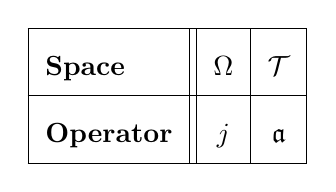
\begin{tikzpicture}
      % Création du tableau dans un nœud
      \node[anchor=east,rectangle,inner sep=0pt,outer sep=0pt]%
      (Tbl) {%
        \renewcommand{\arraystretch}{2}%
        \begin{tabular}{|l||c|c|}%
          \hline%
          \textbf{Space}&$\Omega$ & $\mathcal T$ \\%
          \hline%
          \textbf{Operator} & $j$ & $\mathfrak a$ \\
          \hline
        \end{tabular}%
      };

      % % Positionnement des points d'ancrage des flèches
      % \path (Tbl.north east) -- (Tbl.south east) %
      % node[pos=0.10](Fl_R){}% départ flèche rectangulaire
      % node[pos=0.25](Fl_C){}% départ flèche courbe
      % node[pos=0.75](C_lF){}% pointe flèche rectangulaire
      % node[pos=0.9](R_lF){};% pointe  flèche courbe

      % % % Flèche courbe
      % % \draw[->,line width=.8pt,blue!80](Fl_C) .. controls +(1.5cm,.1cm) and +(1.5cm,-.1cm)..
      % % node[ellips,fill=white,draw]{$\times\,0{,}02$} (C_lF);
      % % % Flèche rectangulaire
      % \draw[<-,line width=.8pt,red!80](Fl_C) -| (2.8cm,0cm)
      % node[circle,fill=white,draw]{sheafification}|-(R_lF) ;
    \end{tikzpicture}

    \end{center}
  }
  \only<3>{
    \begin{center}
      
    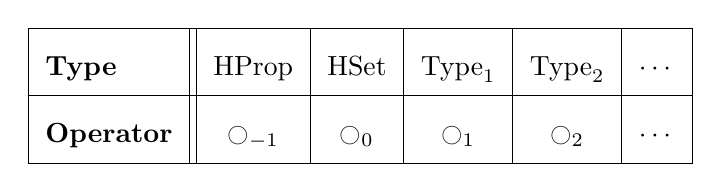
\begin{tikzpicture}
      % Création du tableau dans un nœud
      \node[anchor=east,rectangle,inner sep=0pt,outer sep=0pt]%
      (Tbl) {%
        \renewcommand{\arraystretch}{2}%
        \begin{tabular}{|l||c|c|c|c|c|}%
          \hline%
          \textbf{Type}&$\HProp$ & $\HSet$ & $\Type_1$ & $\Type_2$ & $\cdots$ \\%
          \hline%
          \textbf{Operator} & $\modal_{-1}$ & $\modal_0$ & $\modal_1$
          & $\modal_2$ & $\cdots$ \\
          \hline
        \end{tabular}%
      };

      % % Positionnement des points d'ancrage des flèches
      % \path (Tbl.north east) -- (Tbl.south east) %
      % node[pos=0.10](Fl_R){}% départ flèche rectangulaire
      % node[pos=0.25](Fl_C){}% départ flèche courbe
      % node[pos=0.75](C_lF){}% pointe flèche rectangulaire
      % node[pos=0.9](R_lF){};% pointe  flèche courbe

      % % Flèche courbe
      % \draw[->,line width=.8pt,blue!80](Fl_C) .. controls +(1.5cm,.1cm) and +(1.5cm,-.1cm)..
      % node[ellipse,fill=white,draw]{$\times\,0{,}02$} (C_lF);
      % % Flèche rectangulaire
      % \draw[<-,line width=.8pt,red!80](Fl_R) -| (2.8cm,0cm)
      % node[circle,fill=white,draw]{$\times\,50$}|-(R_lF) ;
    \end{tikzpicture}

    \end{center}
  }
\end{frame}

\begin{frame}
  From a modality on $\HProp$, how can we extend it into a sequence of
  modalities ?

  \bigskip

  \onslide<2>{Inductively~: from a modality $\modal_n$ on $\Type_n$,
    we build a modality $\modal_{n+1}$ on $\Type_{n+1}$.}
\end{frame}

\begin{frame}{Questions}
  
  When generalizing construction in topos, several questions arises:
  \begin{itemize}[<+(1)->]
  \item Do we generalize subobjects as $n$-subobjects (maps with
    $n$-truncated fibers) or $(-1)$-subobjects (embeddings)? \onslide<6>{\textcolor{blue}{Solved}}
  \item The proof involves kernel pair of a surjection. How to
    generalize it ? \only<6>{\textcolor{blue}{Solved}}
  \item Do we use usual image, or a $n$-image arising from
    $n$-connected/$n$-truncated factorization system?
    \onslide<6>{\textcolor{blue}{Solved}}
  \item How to reach not truncated types? \only<6>{\textcolor{red}{In progress}}
  \end{itemize}
\end{frame}

\begin{frame}
  We notice that axioms of a Lawvere-Tierney topology are similar with
  the ones of a truncated modality on $\HProp$.

  \bigskip

  A modality is an operator changing slighlty the truth values of a
  subobject classifier.

  \note{We know that the type of n truncated types defines a subobject classifier}
\end{frame}

\begin{frame}
  \note{ }
  \frametitle{Recall : Modalities}
  We use the same notion of modalities as in the book, but restricted to be on $n$-truncated types.
\begin{defi}
  \label{sec:defin-basic-prop-1}
  Let $n\geq -1$ be a truncation index. A left exact modality at level
  $n$ is the data of
  \begin{enumerate}[(i)]
  \item A predicate $P:\Type_n \to \HProp$
  \item For every $n$-truncated type $A$, a $n$-truncated type
    $\modal A$ such that $P(\modal A)$
  \item For every $n$-truncated type $A$, a map $\eta_A:A \to
    \modal A$
  \end{enumerate}
  such that
  \begin{enumerate}[(i)]
    \setcounter{enumi}{3}
  \item For every $n$-truncated types $A$ and $B$, if $P(B)$ then
    $$\left\{
      \begin{array}{rcl}
        (\modal A \to B) & \to & (A \to B) \\
        f & \mapsto & f \circ \eta_A
      \end{array} \right.$$
    is an equivalence.
  \end{enumerate}
\end{defi}
\end{frame}


\begin{frame}{Requirements}
  \note<2>{We change slightly the last requirement to ask stability by
  dependent product instead of only arrows}
  We want a predicate on $\Type_{n+1}$, which we call {\em sheaf
    property}, satisfying:
  \begin{itemize}
  \item if $\modal_n$ is the identity modality, then everybody should
    be a sheaf
  \item a closed $(-1)$-subobject of a sheaf should be a sheaf
  \item the type of modal $\Type_n$ should be a sheaf
  \item \only<1>{if $T$ is a sheaf, then $X\to T$ should be a sheaf, for any
    $X$}
    \only<2>{if $T:X\to\Type_{n+1}$ such that any $T\,x$ is a sheaf, then $\prod_{x:X} T\,x$
    should be a sheaf.}
  \end{itemize}
\end{frame}

\subsection{Definitions}
\label{sec:definitions}

\begin{frame}[allowframebreaks]{Dense subobject}
  \note{ }
  \begin{defi}
    Let $E$ be a type. The {\em closure} of a subobject of $E$ with
    $m$-truncated homotopy fibers (or $m$-subobject of $E$, for short),
    classified by $\chi : E \to \nType m$, is the $m$-subobject of $E$
    classified by $\modal_m \circ \chi$.

    \note[item]{The closure operator is just postcomposition of characteristic
      with the modality.}

    An $m$-subobject of $E$ classified by $\chi$ is said to be {\em
      closed in $E$} if it is equal to its closure, \ie
    $\chi = \modal_m \circ \chi$.
    \note[item]{$A$ is closed in $E$ if its closure is $E$.}
  \end{defi}

  Practically, a $m$-subobject of $E$ is just $\{e:E ~\&~ \chi~e\}$, and
  its closure is $\{e:E~\&~\modal_m(\chi~e)\}$.
  \framebreak
  \begin{defi}
    Let $E$ be a type, and $\chi:E \to \nType m$. The $m$-subobject of $E$
    classified by $\chi$ is {\em dense} in $E$ when its $\modal_m$-closure
    is equivalent to $\chi_E$, \ie
    % 
    $$\forall e:E,~ \modal_m  (\chi~e) \simeq \one.$$
  \end{defi}

  Practically, a $m$-subobject $A$ of $E$ is dense if, from the $\modal_m$ point of
  view, you cannot make a difference between $A$ and $E$.
  
\end{frame}

\begin{frame}{Restriction}
  \note{ }
  \begin{defi}
    For any type $E$, characteristic map $\chi : E \to \nType m$ and $F:\nType {(n+1)}$, we define
    $$
    \Phi_E^{\chi,m} : (E \to F) \to (\{e:E~\&~\chi~e\} \to F) 
    $$
    % 
    as the map sending an
    arrow $f:E\to F$ to its restriction $f \circ \pi_1$.
  \end{defi}
\end{frame}

\begin{frame}{Sheaves}
  Following the topos-theoretic idea, we use:
  \begin{defi}[Sheaves]
    A type $F$ of $\nType {(n+1)}$ is a {\em $(n+1)$-sheaf} if \onslide<2>{\textcolor{red}{it is
    separated}, and }for any type $E$ and all dense \textcolor{blue}{$(-1)$-subobject}
    $\chi : E \to \nType {(-1)}$, $\Phi_E^{\chi,-1}$ is an
    equivalence. In other words, the dotted arrow exists and is unique.

    $$\xymatrix{
      \{e:E~\&~\chi~e\}  \ar[r]^-f \ar[d]_{\pi_1} & F \\
      E \ar@{-->}[ru]_{\exists !}&
    }$$
  \end{defi}
  \note[item]{Here, we take (-1)-subobjects, because we want every type
    to be a sheaf for the identity modality.}
  \note[item]{The conditions are not satisfied that way; sheaves are
    not stable by dependent products.}
\end{frame}


\begin{frame}{Separated type}
  \begin{defi}[Separated Type]
    A type $F$ in $\nType {(n+1)}$ is {\em separated} if for any type $E$, and
    all dense \textcolor{blue}{$n$-subobject} $\chi : E \to \nType n$,
    $\Phi_E^{\chi,n}$ is an embedding. In other words, the dotted arrow,
    if exists, is unique.

    $$\xymatrix{
      \{e:E~\&~\chi~e\}  \ar[r]^-f \ar[d]_{\pi_1} & F \\
      E \ar@{-->}[ru]_{!}&
    }$$
  \end{defi}
\end{frame}


\begin{frame}{Two steps}
  \note{ }

  We will proceed in two steps: 
  \begin{enumerate}[(i)]
  \item {\em separation:} From any $T$ in $\nType {(n+1)}$, we construct
    its {\em free} separated object $\separated T$.
  \item {\em completion:} We add what is missing for the free 
    separated type to be a sheaf by using closure.
  \end{enumerate}
  \note[item]{Not equivalent with + construction. We define the free
    separated object, while Grothendieck not.}
\end{frame}


\subsection[Separation]{From types to separated types}
\label{sec:from-types-separated}

\begin{frame}{}{Separation}
  \note{ }
  Let $T : \nType {(n+1)}$. We define $\separated T$ as the image of
  $\modal_n^T \circ \{\cdot\}_T$, as in
  $$\xymatrix{
    T \ar[r]^{\{\cdot\}_T} \ar[d]_{\mu_T} & \nType n^T \ar[d]^{\modal_n^T} \\
    \separated T \ar[r]& \left( \nType n^\modal \right)^T
  }$$
  where $\{\cdot\}_T$ is the singleton map $\lambda (t:T),~\lambda
  (t':T),~t=t'$.
  \note{We note that, as $\mu_T$ is the surjection-embedding
    factorization, $\mu_T$ is indeed a surjection.}
  % 
  \pause
  $\separated T$ can be given explicitly by
  % 
  $$
  \begin{array}{rcl}
    \separated T &\defeq & \im (\lambda~t:T,~\lambda~ t',~ \modal_n (t = t')) \\
                 & \defeq & \sum_{u:T \to \nType n^\modal} \left\| \sum_{a:T} 
                            (\lambda t,~\modal_n (a=t)) = u\right\|.
  \end{array}
  $$
\end{frame}

\begin{frame}{}{Separation is a modality}
  \note{ }
  At first, we prove that:
  \note[item]{That's indeed the least we can ask.}
  \begin{prop}
    For any $T:\nType {(n+1)}$, $\separated T$ is separated.  
  \end{prop}
  \pause
  \vspace{1em}
  
  Then, we want
  \note<2>[item]{This actually is the hard part of the construction ;
    especially the universal property for the reflective subuniverse.}
  \begin{thm}
    $(\separated,\mu)$ defines a modality on $\nType {(n+1)}$.
  \end{thm}
\end{frame}

\begin{frame}{Sketch of proof}
  In topoi, the proof goes this way:
  \begin{itemize}[<+(1)->]
  \item $\mu_T$ is a surjection, thus it coequalizes its kernel pair
    $$\xymatrix{
      T \times_{\separated T} T \dar[r]{2pt}^-{\pi_1}_-{\pi_2}& T \ar[r]^-{\mu_T} & \separated T
    }$$
  \item Then $T \times_{\separated T} T = \overline \Delta$, where
    $\Delta = \{(x,y):T^2~\&~x=y\}$. The following is a coequalizer
    $$\xymatrix{
      \overline \Delta\dar[r]{2pt}^-{\pi_1}_-{\pi_2}& T \ar[r]^-{\mu_T} & \separated T
    }$$

  \end{itemize}
\end{frame}
\begin{frame}{Sketch of proof}
  Then, if $Q$ is any separated type and $f:T\to Q$, it makes the diagram
  $$\xymatrix{
    \overline \Delta\dar[r]{2pt}^-{\pi_1}_-{\pi_2}& T \ar[r]^f & Q}$$
  commute, thus $f$ factors through $\separated T$.
\end{frame}

\begin{frame}
  In HoTT, it gets harder. We use the following HITs:
  \only<1,2>{\begin{align*}    
      \KP(f)&\left|
        \begin{array}{lll}
          \kp &:& A\to \KP(f) \\
          \alpha &:& \displaystyle{\prodD {x,y}{A}{f\, x = f\, y \to
              \kp\,x=\kp\,y}}\\
          \alpha_1&:& \displaystyle{\prodD x A {\alpha(x,x,1) = 1}}
        \end{array}
      \right. 
      \\
      \bigskip &
      \\
      \onslide<2->{\mathring T_X&\left|
          \begin{array}{lll}
            \mathring t&:&\|X\|_{n+1} \to \mathring T_X \\
            \mathring \alpha&:& \displaystyle{\prodD{a, b}{\|X\|_{n+1}}{\modal (a=b) \to
                \mathring t(a) = \mathring t(b)}} \\
            \mathring \alpha_1&:&\displaystyle{\prodD a {\|X\|_{n+1}}{
                \mathring \alpha(a , a, \eta_{a=a} 1) = 1}}
          \end{array}
        \right.}
    \end{align*}}

  \only<3>{
    \[ 
  \xymatrix{
    \displaystyle{\sumD{a,b}X {f x = f y}} \ar@<-.5ex>[r]_-{\pi_2}
    \ar@<.5ex>[r]^-{\pi_1} & A \ar@/_2pc/[l]_\delta \ar[r] & \KP(f)
  }
\]
\bigskip
 \[
    \xymatrix{\displaystyle{\sumD {a,b}{\|X\|_{n+1}} {\modal (a=b)}} \ar@<-.5ex>[r]_-{\pi_2} \ar@<.5ex>[r]^-{\pi_1}
      & \|X\|_{n+1}\ar@/_2pc/[l] \ar[r] & \mathring T_X
    }\]
  }
\end{frame}

\begin{frame}
\note<1->[item]{We know that the n+1 colimit of the truncated iterated kernel
  pair of muT is its image, thus the separation of T}
\note<2->[item]{We can prove that the truncated iterated kernel pair
  is equivalent to the iteration of T rings}
\note<3->[item]{Thus the separation of T is the n+1 colimit of the
  bottom diagram}
  \only<2>{\small{
    \[
    \xymatrix{%
     \|\KP^0(\mu_T)\|_{n+1} \ar[r] \ar[d]^*[@]{\hbox to 0pt{\hss$\sim$\hss}}&
     \|\KP^1(\mu_T)\|_{n+1} \ar[r] \ar[d]^*[@]{\hbox to
       0pt{\hss$\sim$\hss}} & 
     \|\KP^2(\mu_T)\|_{n+1} \ar[r] \ar[d]^*[@]{\hbox to
       0pt{\hss$\sim$\hss}} & \cdots \\
     \mathring T_0 \ar[r] & \mathring T_1 \ar[r] &  \mathring T_2
     \ar[r] &\cdots
    }
  \]
  }}
\only<1>{\small{\[
    \xymatrix{%
      & \text{$(n+1)$-colimit} && \\
      &\separated T&& \\
     \|\KP^0(\mu_T)\|_{n+1} \ar[r]  \ar[ur]&
     \|\KP^1(\mu_T)\|_{n+1} \ar[r] \ar[u]& 
     \|\KP^2(\mu_T)\|_{n+1} \ar[r] \ar[ul]& \cdots \ar[ull]\\
    }
  \]}}
\only<3>{\small{
    \[
    \xymatrix{%
     \mathring T_0 \ar[r] \ar[dr] & \mathring T_1 \ar[r]\ar[d] &  \mathring T_2
     \ar[r] \ar[dl]&\cdots \ar[dll]\\
     &\separated T&& \\
     & \text{$(n+1)$-colimit} &&
    }
  \]
  }}
\end{frame}

\subsection[Sheafification]{From separated types to sheaves}
\label{sec:from-separated-sheaves}

\begin{frame}{}{Sheafification}
  \note{ }
  For any $T$ in $\nType {(n+1)}$, 
  $\modal_{n+1}T$ is defined as the closure of $\separated T$,
  seen as a subobject of $T \to \nType n^\modal$. 
  % 
  $\modal_{n+1}T$ can be given explicitly by
  $$
  \modal_{n+1} T \ \defeq \sum_{u:T \to \nType n^\modal} \modal_{-1}\left\| \sum_{a:T} 
    (\lambda t,~\modal_n (a=t)) = u\right\|.
  $$
\end{frame}

\begin{frame}[Sheafification is a lex modality]
  \note{ }
  As above, we first prove that:
  \note[item]{Again, we need this.}
  \begin{prop}
    For any $T:\nType {(n+1)}$, $\modal_{n+1}T$ is a sheaf.
  \end{prop}
  It is true because of the requirement we asked about sheaves:
  \begin{lem}
    Let $X:\nType {(n+1)}$ and $U$ be a sheaf. If $X$ embeds
    in $U$, and is closed in $U$, then $X$ is a sheaf.
  \end{lem}

  \pause
  \vspace{1em}

  Then:
  \begin{thm}
    $(\modal_{n+1},\nu)$ defines a left-exact modality.
  \end{thm}
  \note<2>[item]{This time, it's pretty easy\dots}
\end{frame}

\begin{frame}{Sketch of proof}
  \note{First, we use the universality of separation. Then we use
    universality of closure}
  Let $T,Q:\nType {(n+1)}$ such that $Q$ is a sheaf. Let $f:T\to Q$.
  Because $Q$ is a sheaf, it is in particular separated;
  % 
  thus we can extend $f$ to $\separated f:\separated T\to Q$.
  \pause
  \vspace{1em}

  But as $\modal_{n+1} T$ is the closure of $\separated T$, $\separated T$ is dense
  into $\modal_{n+1} T$, so the sheaf property of $Q$ allows to extend
  $\separated f$ to $\modal_{n+1} f:\modal_{n+1} T \to Q$.

  As all these steps are universal, the composition is.
  \note<3>{again, the modality thing is just technical, and the
    left-exactness comes from the compatibility.}
\end{frame}

\subsection{Summary}
\label{sec:consequences}

\begin{frame}
  From any left-exact modality on $\Type_n$,
  \[\displaystyle{\modal_{n+1} \defeq  \lambda T:\nType {(n+1)}},
  \sum_{u:T \to \nType n^\modal} \modal_{-1} 
  \left\|
    \sum_{a:T} u= (\lambda t,~\modal_n (a=t))
  \right\|\]
  defines a modality on $\Type_{n+1}$.

  \bigskip

  Thus, starting from a modality on $\HProp$, we can build a modality
  on any $\Type_n$ for any $n$.
\end{frame}

\begin{frame}

  \note{ }
  Starting from the left-exact modality $\modal_{-1} P = \lnot\lnot
  P$, when working only with $n$-truncated types, it allows to use the
  law of excluded middle.

\end{frame}

\section{Future works}
\label{sec:fw}
\begin{frame}{Universes}
  \note{Universes are indeed an issue in our construction ; we need to
    use type-in-type even for just the inductive step}
  The construction can be written inductively:
  \[ \begin{array}{l}
    \modal : \forall \ (n : nat), \ \nType n \to \nType n 
    \\
    \bullet~\modal_{-1\phantom{n}} \text{ is a left exact modality on
      $\HProp$} \\
    \bullet~\displaystyle{\modal_{n+1} \defeq  \lambda T:\nType {(n+1)}},\\
    \hspace{5em} \displaystyle{\sum_{u:T \to \nType n^\modal} \modal_{-1} 
      \left\|
        \sum_{a:T} u= (\lambda t,~\modal_n (a=t))
      \right\|}
  \end{array}
  \]

  Here , the universe level increases strictly at each step, hence it is
  impossible to take the fixpoint: we would need universes to be
  indexed by (non-finite) ordinals.

\end{frame}

\begin{frame}{Extension to type}
  The modalities are defined just for truncated type.

  \bigskip

  How to extend it to all types ?
  \note{We know that there are non-truncated types. In a general
    setting, some types are not even the limit of their successive truncations}
\end{frame}

\begin{frame}
  \begin{itemize}
  \item<1-> First idea: Write any type as the limit of its
    truncation. \onslide<2->{\textcolor{red}{False !}}
  \item<3-> Second idea: Suppose that every type is the limit of
    its truncations, and use Postnikov towers
    \[ T = T_\infty \to \cdots \to \|T\|_0 \to \|T_{-1}\|.\]
    But
    \[  \cdots \to \modal_0\|T\|_0 \to \modal_{-1} \|T_{-1}\|\]
    is not a Postnikov pretower, because
    \[  \left\|\modal_{n+1} \|T\|_{n+1}\right\|_{n} \not= \modal_n
    \|T\|_n.\]
    \onslide<4->{\textcolor{red}{False !}}
  \end{itemize}
\end{frame}

\begin{frame}[allowframebreaks]
  \frametitle{Translation}
  \begin{itemize}
  \item For types
    \[
    \begin{array}{lcl}
      \left[ \Type\right] &\defeq& (\Type^\modal,\pi_{\Type^\modal})
    \end{array}
    \]
    where $\pi_{\Type^\modal}$ is a proof that $\Type^\modal$ is itself
    modal.
    To ease the reading in what follows, we introduce the notation  \[ 
    \Lbrack A \Rbrack \defeq \pi_1 \left[ A \right]\]

  \item For dependent sums
    \[
    \begin{array}{lcl}
      \left[ \sumD x A B \right] &\defeq&  \left( \sumD x{\Lbrack A \Rbrack}
        {\Lbrack B\Rbrack} , \pi_\Sigma^{[A],[B]}
      \right)\\[0.5em]
      \left[  (x,y)\right] &\defeq& ([x],[y]) \\[0.5em]
      \left[  \pi_i t\right] &\defeq& \pi_i [t] \\[0.5em]
    \end{array}
    \]
    where $\pi_{\Sigma}^{A,B}$ is a proof that $\sumD x A B$ is modal when
    $A$ and $B$ are.
  \item For dependent products
    \[
    \begin{array}{lcl}
      \left[ \prod_{x:A} B \right] &\defeq& \left( \prod_{x:\Lbrack A \Rbrack}
        \Lbrack B\Rbrack , \pi_{\Pi}^{[A],[B]}
      \right)\\[0.5em]
      \left[  \lambda\, x:A,~M \right] &\defeq&\lambda\,x:\Lbrack A
      \Rbrack,~[ M ]
      \\[0.5em]
      \left[ t \, t' \right] &\defeq& [t] [t'] \\[0.5em]
    \end{array}
    \]
    where $\pi_{\Pi}^{A,B}$ is a proof that $\prodD x A B$ is modal when $B$ is.
  \item For paths
    \[
    \begin{array}{lcl}
      \left[  x=_A y \right] &\defeq& \left( [x] =_{\Lbrack A\Rbrack} [y] , \pi_=^{[x],[y]}
      \right)\\[0.5em]
      \left[ 1 \right] &\defeq& 1\\[0.5em]
      \left[ J \right] &\defeq& J \\[0.5em]
    \end{array}
    \]
    where $\pi_{=}^{x,y}$ is a proof that $x=_A y$ is modal when $A$ is.
  \item For positive types (we only treat the case of the sum as an example)
    \[
    \begin{array}{lcl}
      \left[  A+B \right] &\defeq& \left( \modal(\Lbrack A \Rbrack + \Lbrack B
        \Rbrack); \pi_\modal(\Lbrack A \Rbrack + \Lbrack B
        \Rbrack)\right)\\[0.5em]
      \left[  \mathrm{in}_\ell t \right] &\defeq& \eta (\mathrm{in}_\ell [t]) \\[0.5em]
      \left[  \mathrm{in}_r t \right] &\defeq& \eta (\mathrm{in}_r [t]) \\[0.5em]
      \left[ \langle f ,g\rangle\right] &\defeq& \modal_{\mathrm{rec}}^{\Lbrack A\Rbrack +
        \Lbrack B\Rbrack} \langle
      [f],[g]\rangle\\[0.5em]
    \end{array}
    \]
  \item For truncations ($i\leqslant n$)
    \[
    \begin{array}{lcl}
      \left[  \|A\|_i \right] &\defeq& (\modal \| \Lbrack A\Rbrack  \|_i;
      \pi_\modal(\| \Lbrack A\Rbrack
      \|_i)) \\[0.5em]
      \left[ |t|_i \right] &\defeq& \eta |[t]|_i \\[0.5em]
      \left[ |f|_i \right] &\defeq& \modal_{\mathrm{rec}}^{\| \Lbrack
        A\Rbrack  \|_i} | [f] |_i
    \end{array}
    \]

  \end{itemize}
\end{frame}

\end{document}
